%%%%%%%%%%%%%%%%%%%%%%%%%%%%%%%%%%%%%%%%%
% Short Sectioned Assignment
% LaTeX Template
% Version 1.0 (5/5/12)
%
% This template has been downloaded from:
% http://www.LaTeXTemplates.com
%
% Original author:
% Frits Wenneker (http://www.howtotex.com)
%
% License:
% CC BY-NC-SA 3.0 (http://creativecommons.org/licenses/by-nc-sa/3.0/)
%
%%%%%%%%%%%%%%%%%%%%%%%%%%%%%%%%%%%%%%%%%

%----------------------------------------------------------------------------------------
%	PACKAGES AND OTHER DOCUMENT CONFIGURATIONS
%----------------------------------------------------------------------------------------

\documentclass[11pt,a4paper]{article} % A4 paper and 11pt font size
\usepackage[utf8]{inputenc} %ISO-8859-2
\usepackage[T1]{fontenc} % Use 8-bit encoding that has 256 glyphs
%\usepackage{fourier} % Use the Adobe Utopia font for the document - comment this line to return to the LaTeX default
\usepackage[polish]{babel} % English language/hyphenation
\usepackage{amsmath,amsfonts,amsthm} % Math packages
\usepackage{changepage}	

\usepackage{lipsum} % Used for inserting dummy 'Lorem ipsum' text into the template
\usepackage{morefloats}
\usepackage{multicol}
\usepackage[section]{placeins}
\usepackage[font=small,labelfont=bf,justification=centering]{caption}
\usepackage[a4paper]{geometry}
\usepackage{hyperref}
\usepackage{dirtytalk}

\usepackage{color}
 
\definecolor{codegreen}{rgb}{0,0.6,0}
\definecolor{codegray}{rgb}{0.5,0.5,0.5}
\definecolor{codepurple}{rgb}{0.58,0,0.82}
\definecolor{backcolour}{rgb}{0.95,0.95,0.92}
\usepackage{listings}
\lstdefinestyle{mystyle}{
    backgroundcolor=\color{white},   
    commentstyle=\color{codegreen},
    keywordstyle=\color{blue},
    numberstyle=\tiny\color{codegray},
    stringstyle=\color{codepurple},
    % basicstyle=\footnotesize,
    breakatwhitespace=false,         
    breaklines=true,                 
    captionpos=b,                    
    keepspaces=true,                  
    numbersep=5pt,                  
    showspaces=false,                
    showstringspaces=false,
    showtabs=false,                  
    tabsize=2
}
 
\lstset{style=mystyle}
% \lstset{basicstyle=\footnotesize\ttfamily,breaklines=true}


%\usepackage{sectsty} % Allows customizing section commands
%\allsectionsfont{\centering \normalfont\scshape} % Make all sections centered, the default font and small caps

%\usepackage{fancyhdr} % Custom headers and footers

\usepackage[pdftex]{graphicx}
\def\code#1{\texttt{#1}}
\usepackage{inconsolata}

%\usepackage[]{algorithm2e}

%\pagestyle{fancyplain} % Makes all pages in the document conform to the custom headers and footers
%\fancyhead{} % No page header - if you want one, create it in the same way as the footers below
%\fancyfoot[L]{} % Empty left footer
%\fancyfoot[C]{} % Empty center footer
%\fancyfoot[R]{\thepage} % Page numbering for right footer
%\renewcommand{\headrulewidth}{0pt} % Remove header underlines
%\renewcommand{\footrulewidth}{0pt} % Remove footer underlines
%\setlength{\headheight}{13.6pt} % Customize the height of the header

\numberwithin{equation}{section} % Number equations within sections (i.e. 1.1, 1.2, 2.1, 2.2 instead of 1, 2, 3, 4)
\numberwithin{figure}{section} % Number figures within sections (i.e. 1.1, 1.2, 2.1, 2.2 instead of 1, 2, 3, 4)
\numberwithin{table}{section} % Number tables within sections (i.e. 1.1, 1.2, 2.1, 2.2 instead of 1, 2, 3, 4)

%\setlength\parindent{0pt} % Removes all indentation from paragraphs - comment this line for an assignment with lots of text

%----------------------------------------------------------------------------------------
%	TITLE SECTION
%----------------------------------------------------------------------------------------

\newcommand{\horrule}[1]{\rule{\linewidth}{#1}} % Create horizontal rule command with 1 argument of height

\title{
\normalfont \normalsize
\textsc{Politechnika Warszawska \\Wydział Elektroniki i Technik Informacyjnych} \\ [25pt] % Your university, school and/or department name(s)
% \horrule{0.5pt} \\[0.4cm] % Thin top horizontal rule
\Large Przetwarzanie cyfrowe obrazów\\
\huge Rozpoznawanie loga sieci Tesco - sprawozdanie \\ % The assignment title
\horrule{1pt} \\[0.5cm] % Thick bottom horizontal rule
}

\author{Michał Dziekoński} % Your name

\date{\normalsize\today} % Today's date or a custom date

\begin{document}

\maketitle % Print the title

\section{Temat projektu}

Dla  indywidualnie  wybranej  klasy  obrazów  dobrać,  zaimplementować i  przetestować odpowiednie procedury wstępnego przetworzenia, segmentacji, wyznaczania   cech oraz identyfikacji obrazów cyfrowych. Powstały w wyniku projektu program powinien poprawnie rozpoznawać wybrane obiekty dla reprezentatywnego zestawu obrazów wejściowych.

Wybrana klasa obrazów to zdjęcia zawierające logo sieci hipermarketów Tesco - czerwony tekst składający się z kolejno ułożonych liter T, E, S, C, O. Zestaw obrazów składa się z pięciu plików, z czego na każdym z nich znajdują się przynajmniej dwa fragmenty do rozpoznania.

\section{Kompilacja i instrukcja uruchomienia}

\subsection{Kompilacja}

Kompilacja programu jest możliwa za pomocą dwóch programów:
\begin{itemize}
	\item CMake - komendy \textbf{cmake} i \textbf{make} (kompatybilne z CLion)
	\item Scons - komenda \textbf{scons} (możliwe do uruchomienia z terminala, buduje program do pliku \textbf{build/run})
\end{itemize}

Do kompilacji wymagany jest kompilator wspierający opcję \textbf{C++1z} (wymagane wsparcie dla "Nested namespace definition"). Kompilatory wspierające tę opcję to:
\begin{itemize}
	\item GCC w wersji 6.0.0
	\item Clang w wersji 3.6
	\item MSVC w wersji 14.3
\end{itemize}

Do kompilacji wymagana jest również biblioteka OpenCV w wersji co najmniej 3.2.0, zainstalowana na stałe w systemie operacyjnym.

\subsection{Instrukcja obsługi}

Program uruchamiany z okna terminala przyjmuje następujące opcje:
\begin{itemize}
	\item \textbf{--file=FILEPATH} (wymagany) - ścieżka do pliku obrazu z rozpoznawanym obrazem
	\item \textbf{--binary} (opcjonalny) - flaga przełączająca tryb wyświetlania wyniku z obrazka oryginalnego na obrazek binarny (po operacji binaryzacji)
\end{itemize}

\section{Opis działania projektu}

Program stworzony na potrzeby projektu ma za zadanie wykonać serię operacji na wcześniej załadowanym obrazie w celu wykrycia fragmentów zawierających logo Tesco. Ogólną sekwencję działania procesu rozpoznawania można opisać następująco:
\begin{enumerate}
	\item Wstępna obróbka obrazu - wstępne polepszenie jakości obrazu w kontekście rozpoznawania, ma na celu uwydatnić cechy przydatne w dalszej obróbce lub usunąć zakłócenia negatywnie wpływające na ten proces.
	\item Binaryzacja obrazu - transformacja obrazu kolorowego do postaci binarnej, gdzie elementy znaczące w punktu widzenia dalszego przetwarzania są koloru białego, pozostałe są czarne.
	\item Obróbka obrazu binarnego - obraz w postaci binarnej pozwala na wykonanie pewnych dodatkowych transformacji, które dodatkowo mogą usprawnić proces rozpoznawania. W tym kroku możliwe są np. operacje poprawiania konturów elementów obrazu.
	\item Segmentacja - jest to wstępne grupowanie pikseli obrazu w segmenty składające się na większe, jednolite obiekty sceny.
	\item Wstępna filtracja - ponieważ pewne grupy pikseli nie stanowią żadnych znaczących z punktu widzenia rozpoznawania obrazów elementów (np. obiekty tła, które przeszły przez proces binaryzacji razem z właściwymi obiektami do rozpoznania), przed uruchomieniem właściwego rozpoznawania warto z góry usunąć fragmenty, które na pewno nie będą składać się na rozpoznawany fragment.
	\item Detekcja poszukiwanych fragmentów - ostatni krok polegający na dopasowaniu znalezionych obiektów do siebie w taki sposób, by sprawdzić czy tworzą razem spójną całość, i tym samym są (lub nie) obiektem który mamy rozpoznać w scenie.
\end{enumerate}


\subsection{Wstępna obróbka obrazu}

W pierwszym kroku sprawdzono, czy obrazy wejściowe wymagają jakiejkolwiek obróbki wstępnej. W ramach wyostrzania obrazów zastosowano filtr Unsharp Mask. Okazało się jednak, że żadne ze zdjęć nie wymaga stosowania tego filtru (dla żadnego zdjęcia nie osiągnięto ani poprawy, ani pogorszenia jakości w dalszym rozpoznawaniu obrazu). Obrazy wykorzystane w testach były już ostre, więc nie wymagały dodatkowego ulepszania.

\subsection{Binaryzacja obrazu}

Kolejnym krokiem była binaryzacja obrazu. Ponieważ zadanie polegało na rozpoznawaniu czerwonego teksu, naturalnym pierwszym wyborem było zastosowanie prostego progowania obrazu za pomocą doświadczalnie otrzymanych wartości dla każdej ze składowych. Okazało się jednak, że nie wszystkie zdjęcia mają tą samą barwność tekstu zawartego w logo, przez co nie udało się uzyskać ogólnego progu dla wszystkich próbek.

Znacznie lepsze rezultaty dało wykorzystanie miksera kolorów do kanału monochromatycznego - dla każdego z kanału kolorów udało się dobrać takie współczynniki, które pozwoliły wyodrębnić interesujące informacje, porzucając jednocześnie szum tła. Po mieszaniu kolorów zastosowano proste progowanie w skali szarości.

\subsection{Obróbka obrazu binarnego}

Następny krok polegał na dodatkowym wyostrzeniu konturów obiektów sceny. W ramach eksperymentów zastosowano dwa przekształcenia - erozję oraz dylację, które w teorii powinny poprawić kontury obiektów oraz wypełnić wszelkie ewentualne ubytki w obiektach.

Okazało się jednak, że nie wszystkie obrazy dobrze "reagują" na takie przekształcenia. Ze względu na to, że niektóre fragmenty obrazów były stosunkowo małe, transformacje doprowadzały do odwrotnego efektu niż zamierzony - zamiast poprawiać kontury, usuwały piksele niszcząc kształty obiektów. Ponieważ pierwotne kontury były na tyle dobre by móc kontynuować proces rozpoznawania, transformacje dylacji i erozji zostały wyłączone.

\subsection{Segmentacja}

Przygotowany obraz binarny został następnie poddany procesowi segmentacji, czyli grupowania pikseli w spójne obszary. Wykorzystano do tego algorytm Floodfill, który dla każdego białego piksela starał się odpowiednio "zalać" danym identyfikatorem jego sąsiadów, tworząc przez to zgrupowanie pikseli. Wykorzystana implementacja algorytmu Floodfill korzysta z ręcznie przygotowanego stosu na "przeszukiwanych sąsiadów" głównie ze względu na to, że standardowa wersja rekurencyjna znacznie spowalniała działanie programu, a dla większych obrazów mogła wywoływać błędy braku pamięci operacyjnej. Każda grupa pikseli została na końcu zapakowana do kontenera przechowującego zarówno same piksele, jak i tzw. Bounding Box całego obszaru.

\begin{figure}
	\centering
	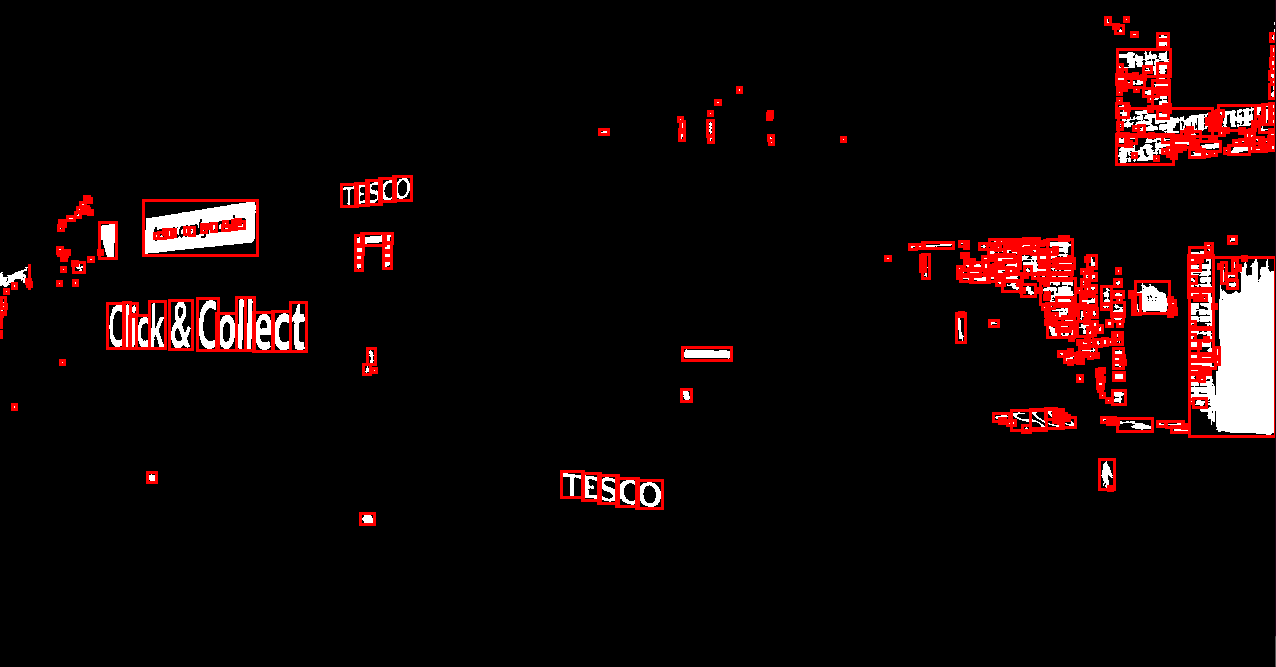
\includegraphics[width=14cm]{pobr_proj_seg1.png}
	\caption{Przykład segmentacji obrazu.}
	\label{fig:pobr_proj_seg1}
\end{figure}


\subsection{Wstępna filtracja}

Kolejnym etapem było filtrowanie niechcianych obiektów ze sceny. W pierwszym kroku nastąpiła eliminacja obiektów które są zbyt małe lub zbyt duże jak na litery loga. W drugiej części sprawdzane były niezmienniki momentowe segmentów (od M1 do M7), które ze względu na swoje właściwości pozwalają wykrywać podobne elementów, niezależnie od ich skalowania czy obrotu. W ramach eksperymentów wyznaczono przedziały wartości tych niezmienników, w których można było stwierdzić czy dany segment należy do np. klasy liter T lub S. Wszystkie inne obiekty, których niezmienniki nie znajdowały się w odpowiednich przedziałach, były odrzucane.

\subsection{Detekcja poszukiwanych fragmentów}

Ostatnim krokiem było rozpoznanie i stwierdzenie, czy wykryte segmenty zawierające litery są poprawnie ułożone i stanowią w swoim obrębie logo Tesco. Jako "kontur" podstawowy zostały wykorzystane litery T i O, ponieważ leżą na skraju loga. Program sprawdza wszystkie możliwe kombinacje wykrytych liter T i O, próbuje dopasować je do jednego fragmentu (sprawdzając, czy odległość między ich środkami pozwala na umieszczenie wewnątrz mniej więcej trzech dodatkowych liter E, S, C). Jeśli to się powiedzie, program stara się znaleźć pasujące w przewidywane miejsca kolejne, wewnętrzne litery wyrazu. W przypadku dopasowania wszystkich pięciu liter tworzony jest nowy segment, stanowiący Bounding Box dla całego loga Tesco.

\begin{figure}
	\centering
	
\includegraphics[width=14cm]{pobr_proj_bin1.png}
	\caption{Przykład ostatecznego wyniku rozpoznawania loga Tesco. Obraz zawiera 11 rozpoznanych fragmentów, wyświetlany jest w formacie binarnym.}
	\label{fig:pobr_proj_bin1}
\end{figure}

\section{Wnioski}

Zgodnie z założeniami, projekt rozpoznaje wszystkie poprawne wystąpienia loga sieci Tesco na wszystkich obrazach z zestawu testowego. Na niektórych zdjęciach znajdują się również fragmentaryczne loga (np. naderwana część pudełka, zasłaniająca jedną z liter), które choć w fazie segmentacji i filtracji zostały poprawnie rozpoznane jako fragmenty całości loga, tak w ostatecznej fazie nie zostały uznane za pełne logo (co jest zgodne z oczekiwaniami - tylko logo zawierające wszystkie litery w poprawnej kolejności zostanie oznaczone jako pełny segment loga).

Binaryzacja obrazu z wykorzystaniem miksera kolorów okazała się znacznie lepszą metodą niż progowanie kolorów. Pozwoliła na znacznie lepsze wyodrębnienie właściwych fragmentów loga przy jednoczesnym wyeliminowaniu mniejszych lub większych anomalii będących składnikami tła. Podczas eksperymentów, przejście na binaryzację mikserem pozwoliło znacznie skrócić czas wykonywania programu w dalszych fazach. Dodatkowym atutem było również uniezależnienie się od operatorów poprawy jakości, czy to w fazie wstępnej (kolorowy obrazek) czy w fazie binarnej - mikser, w przeciwieństwie do progowania kolorów, nie wprowadzał znacznych anomalii na krawędziach czy wewnątrz obiektów, dzięki czemu obyło się bez użycia operacji morfologicznych do poprawy kształtów obiektów.

Potencjalnym polem do rozwoju projektów (również interdyscyplinarnie) jest klasyfikacja liter. W tym projekcie rozpoznawanie przynależności do danej klasy (np. litery T) jest oparte na prostym systemie zakresowym, gdzie każda litera ma określony eksperymentalnie zakres wartości współczynników momentowych. Tak wyznaczone zakresy naturalnie nie będą pasowały do większych próbek testowych, gdzie może okazać się że klasy i ich ograniczenia wartościowe są nadmiernie dopasowane do początkowego zestawu testowego. Przy większym, oznakowanym zbiorze testowym można by zastosować np. naiwny klasyfikator Bayesowski do automatycznego wyznaczenia poprawnych przedziałów, dla zbiorów nieoznakowanych można by podjąć próbę wykorzystania algorytmów klastrujących jako formę uczenia bez nadzoru.

\end{document}
